\documentclass[11pt]{article}

\usepackage[letterpaper,margin=1in]{geometry}
\usepackage{graphicx}
\usepackage{booktabs}
\usepackage{amsmath}
\usepackage{amssymb}
\usepackage{xcolor}
\usepackage{caption}
\usepackage{enumitem}
\usepackage[T1]{fontenc}
\usepackage{lmodern}
\usepackage[colorlinks=true,linkcolor=black,citecolor=black,urlcolor=blue!60!black]{hyperref}

\captionsetup{font=small,labelfont=bf}
\setlist{itemsep=2pt,topsep=4pt,parsep=0pt}
\newcommand{\wga}{\textsc{wga}}
\emergencystretch=3em
\sloppy
\renewcommand{\topfraction}{0.92}
\renewcommand{\bottomfraction}{0.7}
\renewcommand{\textfraction}{0.07}
\renewcommand{\floatpagefraction}{0.85}
\setcounter{topnumber}{2}
\setcounter{totalnumber}{3}

\title{\vspace{-1.5em}Does Model Compression Undo Robustness?\\
\large Group robustness of compressed vision transformers,\\
and whether data pruning survives deployment}

\author{Anusha Upadhyay \and Shreyas Visweshwaran \and Swasti Sadanand}
\date{Advisor: Prof.\ Jung-Eun Kim \\[0.4em] \today}

\begin{document}
\maketitle

\vspace{-1.5em}
\begin{center}
\fbox{\begin{minipage}{0.92\textwidth}
\small This plan covers the scope approved on 7 September 2025: \emph{both} the
first phase (compression vs.\ group robustness) and the second phase (does the
robustness bought by data pruning survive compression). Phase~1 is complete and
its results are reported in \S3. Phases~2 and~3 are specified in \S4--\S5.
\end{minipage}}
\end{center}

\section{Approved scope}

The question is whether the two things we routinely do to a model in sequence ---
first make it robust, then make it small --- interact badly. A robustified model
is compressed before deployment, and we want to know whether that second step
silently undoes the first: whether worst-group accuracy degrades faster under
compression than average accuracy does, so that a model still looking healthy on
top-1 has quietly returned to relying on the spurious feature.

Two phases were approved:

\begin{description}[leftmargin=1.6em,style=nextline]
\item[Phase 1] Fine-tune ViT-S/16 on Waterbirds, apply post-hoc compression
(attention-head pruning, FFN neuron pruning, unstructured magnitude pruning, and
weight quantization) with no retraining afterwards, and measure worst-group
against average accuracy.
\item[Phase 2] Apply the data pruning of Mulchandani and Kim (ICLR 2025)
\emph{before} compression, and test whether the robustness it buys survives.
\end{description}

We add a third phase, \S5, which the original proposal committed to
conditionally: if Phase~1 found a robustness gap, we would test a fix by
recomputing core-feature difficulty on the compressed model rather than the dense
one. Phase~1 found the gap, so the condition is met.

\section{Setup}

\begin{table}[h]
\centering
\footnotesize
\begin{tabular}{@{}ll@{}}
\toprule
Model & \texttt{vit\_small\_patch16\_224} (timm), ImageNet-pretrained, 2-way head \\
Data & Waterbirds v1.0, official splits, read directly from \texttt{metadata.csv} \\
Training & Plain ERM, 10 epochs, AdamW $\text{lr}=10^{-5}$, cosine, batch 32 \\
Selection & Best \emph{validation average} accuracy (seed 0: epoch 3) \\
Compression & Applied to the trained checkpoint, evaluated immediately, \textbf{never retrained} \\
Scope & In-block Linear weights only: \texttt{attn.qkv}, \texttt{attn.proj},
\texttt{mlp.fc1}, \texttt{mlp.fc2} (21{,}233{,}664 params) \\
\bottomrule
\end{tabular}
\end{table}

Four groups, indexed $g = 2y + \text{background}$: \texttt{landbird\_on\_land}
(majority, $n_{\text{train}}=3498$), \texttt{landbird\_on\_water} (minority, 184),
\texttt{waterbird\_on\_land} (minority, 56), \texttt{waterbird\_on\_water}
(majority, 1057). The two minority groups are the ones that \emph{conflict} with
the background shortcut.

\subsection*{Three choices that decide what this measures}

\textbf{Training is deliberately group-blind.} No reweighting, no balanced
sampler, no GroupDRO. The model is \emph{supposed} to learn the background
shortcut --- if training were group-balanced, worst-group accuracy would start
high and the experiment would measure nothing.

\textbf{Model selection is on validation average accuracy, never worst-group.}
Selecting on worst-group is itself a group-aware intervention; it would inflate
the ERM baseline and void the premise. Adjusted-average selection is out for the
same reason --- the adjustment weights need group labels, so using it would leak
group information into a pipeline meant to have none.

\textbf{No retraining after compression.} Fine-tuning afterwards lets the model
re-fit the shortcut, and answers a different question.

Throughout, \texttt{acc\_adj\_avg} is per-group accuracy reweighted by
\emph{training} frequency. Waterbirds' val/test splits are far more
group-balanced than train, so a plain test-set mean is not the ${\sim}97\%$
figure quoted in the literature; the adjusted average is.

\section{Phase 1: results (complete)}

Baseline, uncompressed, seed 0: \textbf{98.2\% adjusted average, 70.4\%
worst group}, a gap of 27.8 points. Twenty-nine compression configurations were
evaluated against that checkpoint; thirty-one validation gates guard the
pipeline.

\begin{table}[h]
\centering
\small
\begin{tabular}{@{}lrrrr@{}}
\toprule
Configuration & Sparsity & Adjusted avg & Worst group & Gap \\
\midrule
uncompressed                 & 0.000 & 98.2\%          & 70.4\%          & 27.8 \\
quantize 8-bit, per-channel  & 0.014 & 98.2\% ($-0.0$) & 70.4\% ($-0.0$) & 27.8 \\
quantize 6-bit, per-tensor   & 0.190 & 97.8\% ($-0.4$) & 62.6\% (\textbf{$-7.8$})  & 35.2 \\
magnitude, 30\%              & 0.300 & 97.5\% ($-0.8$) & 54.4\% (\textbf{$-16.0$}) & 43.1 \\
quantize 4-bit, per-channel  & 0.232 & 97.1\% ($-1.2$) & 60.6\% (\textbf{$-9.8$})  & 36.5 \\
remove 6 of 72 heads         & 0.028 & 96.5\% ($-1.7$) & 48.1\% (\textbf{$-22.3$}) & 48.4 \\
FFN, 30\% of neurons         & 0.200 & 83.3\% ($-14.9$)& \phantom{0}2.5\% ($-67.9$) & 80.9 \\
\bottomrule
\end{tabular}
\caption{Compression at matched sparsity costs far more worst-group accuracy than
average accuracy. Deltas are against the uncompressed baseline, in points.}
\end{table}

\textbf{The headline.} Pruning 30\% of the transformer's weights costs
\textbf{0.8 points} of adjusted average accuracy and \textbf{16.0 points} of
worst-group accuracy --- a 21$\times$ difference. An evaluation reporting only
average accuracy would call that compression free. Removing \textbf{6 attention
heads out of 72}, 2.8\% of the targeted weights, costs 1.7 points of average
accuracy and \textbf{22.3 points} of worst-group accuracy.

\begin{figure}[tbp]
\centering
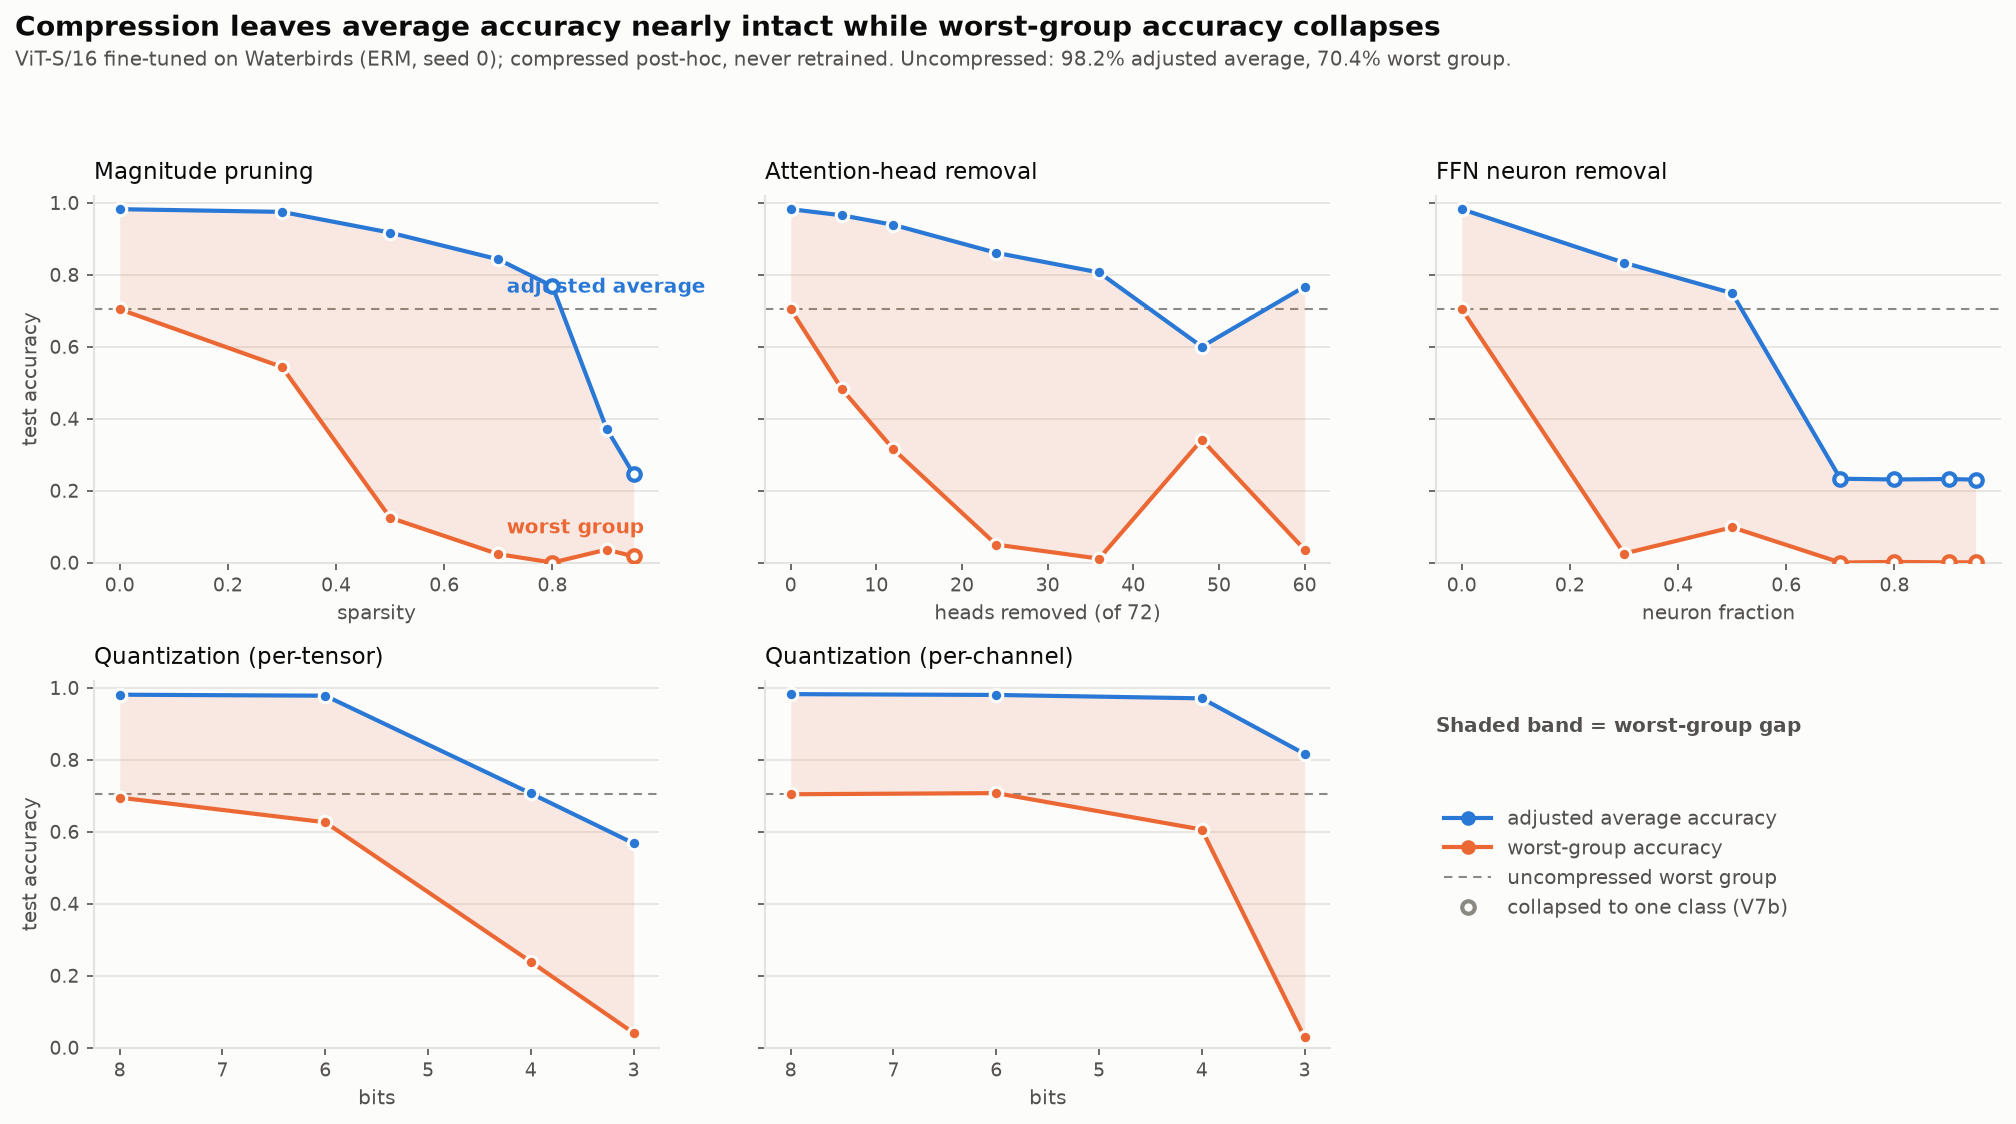
\includegraphics[width=\textwidth]{figures/fig1_avg_vs_worst_group.png}
\caption{Average vs.\ worst-group accuracy across all five compression families.
The shaded band is the gap; it widens everywhere. Hollow markers are
configurations where the model has collapsed to a single predicted class.}
\end{figure}

\begin{figure}[tbp]
\centering
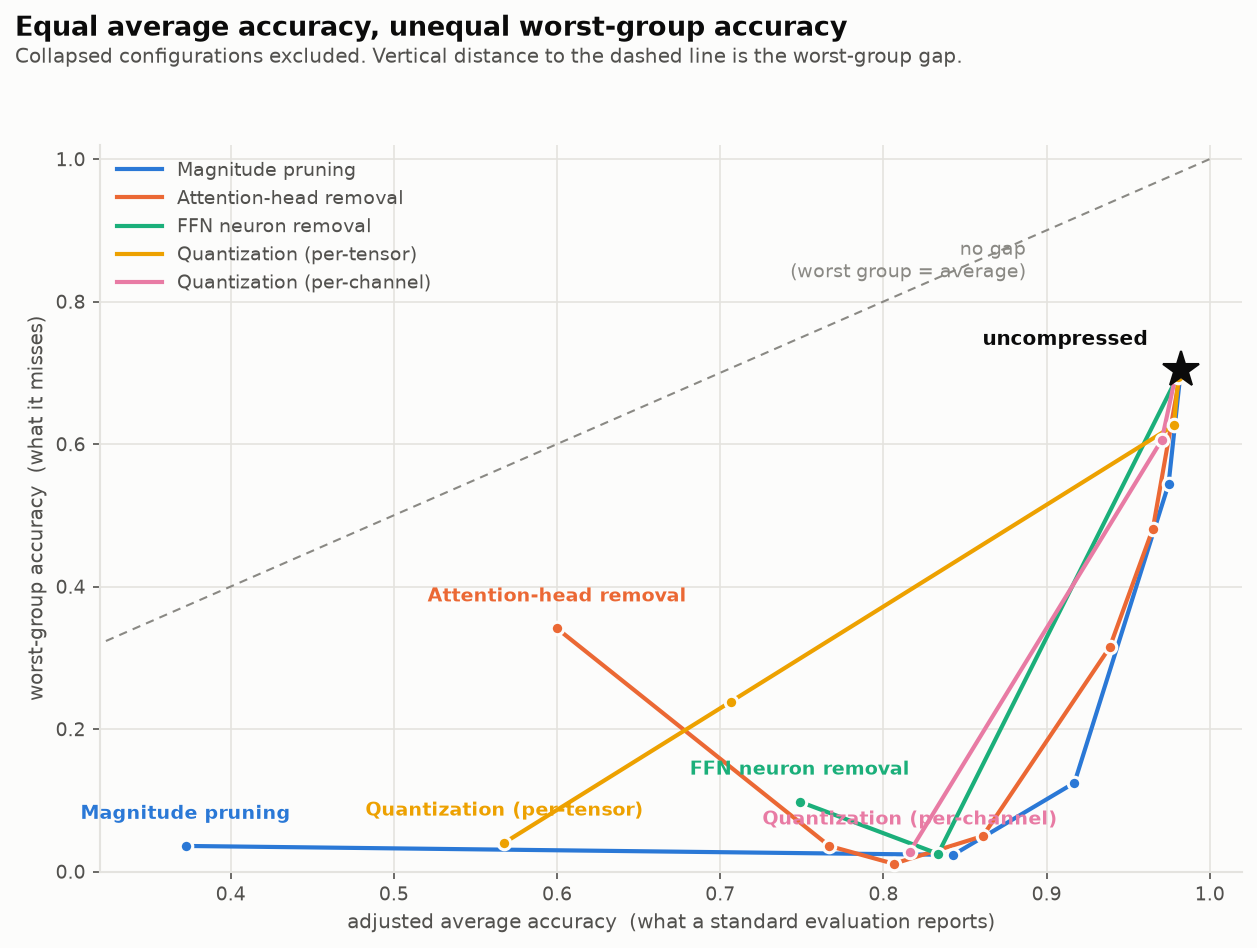
\includegraphics[width=0.62\textwidth]{figures/fig2_tradeoff.png}
\caption{Worst-group plotted against average accuracy, so methods are comparable
at equal average accuracy despite non-commensurable knobs. Collapsed
configurations are excluded.}
\end{figure}

\begin{figure}[tbp]
\centering
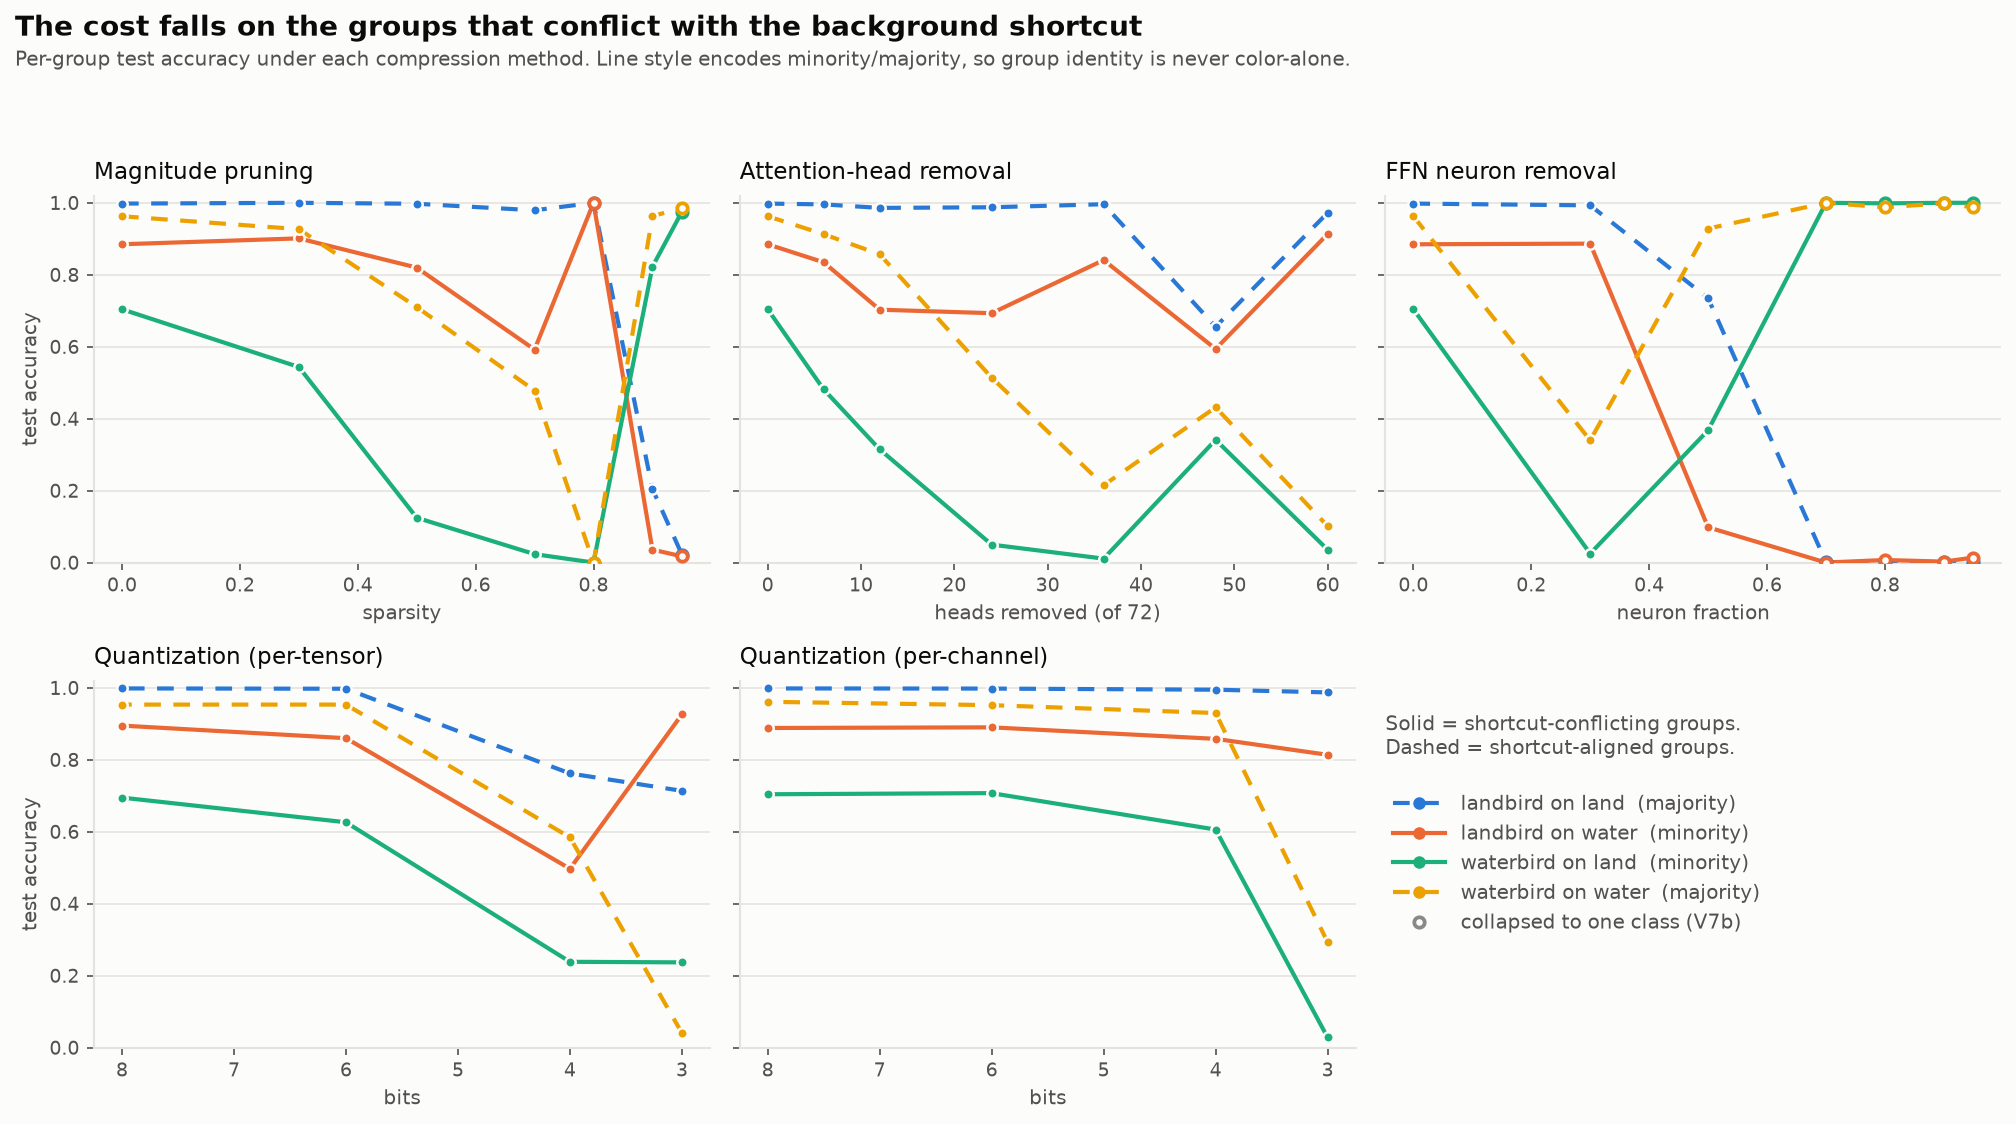
\includegraphics[width=\textwidth]{figures/fig3_per_group.png}
\caption{Which groups pay. \texttt{landbird\_on\_land} --- the majority group
aligned with the shortcut --- holds near 100\% throughout, while
\texttt{waterbird\_on\_land}, the 56-sample conflicting minority, collapses
first.}
\end{figure}

\subsection*{Two things in this data that are easy to misread}

\textbf{The gap narrows again at extreme compression, and that is not robustness
returning.} Past roughly 80\% magnitude sparsity or 70\% FFN removal the model
collapses to predicting a single class. Accuracy is still well-defined, but a
model with one output has no group disparity left to measure. Those points are
detected by the \texttt{pred\_mean} collapse gate, drawn hollow in every figure,
and excluded from the trade-off plot.

\textbf{Head removal is not monotonic.} Removing 48 heads scores \emph{better} on
worst-group (34.1\%) than removing 36 (1.1\%), then falls again at 60. Global
magnitude ranking does not remove heads in order of behavioral importance, and
near-degenerate models reshuffle which group is worst. The deep end of the head
sweep is noise around a collapsed model, not signal.

\textbf{Quantization granularity matters more than bit width.} Per-channel 4-bit
keeps 60.6\% worst-group; per-tensor 4-bit keeps 23.8\%. Same bit budget, very
different outcome.

\section{Phase 2: does data pruning survive compression?}

Phase~1 establishes that compression damages the worst group disproportionately
on a model that was never made robust in the first place. Phase~2 asks the
question that matters for deployment: if we \emph{do} make the model robust
first, does compression take it back?

\subsection{The intervention}

We use the data pruning of Mulchandani and Kim, \emph{Severing Spurious
Correlations with Data Pruning} (ICLR 2025). Its premise is that spurious
correlations are learned primarily because of a handful of training samples whose
\emph{core} feature is hard to learn: where the core feature is hard, the network
prefers the simpler spurious one. Removing those samples severs the dependency,
with no group labels, no inferred domain knowledge, and no human intervention ---
which is exactly what our group-blind pipeline requires.

Sample difficulty is the L2 distance between the network's predicted distribution
and the one-hot label, read from a single ERM run at a fixed early epoch:
\[
  d_i \;=\; \bigl\lVert\, p(w_e, x_i) - y_i \,\bigr\rVert_2 ,
\]
with $e = 1$ for Waterbirds in the original work. Samples are ranked by $d_i$, the
\emph{hardest} are removed class-balanced, and the network is retrained from
scratch on what remains.

Two deviations from the paper, both deliberate and both to be stated in any
write-up. The paper's Waterbirds experiments use an ImageNet-pretrained
ResNet-50; we use ViT-S/16, because the architectural question --- whether
robustness degrades faster when attention heads are removed than when FFN neurons
are --- is the contribution and requires a transformer. And we hold the training
recipe fixed at our Phase~1 recipe rather than the paper's, so that the ERM and
pruned models differ in exactly one thing: the training set.

\subsection{What we add to the pipeline}

Phase~1's code is reusable almost entirely; the compression methods, metrics,
caching, and sweep harness do not change. Five additions are needed:

\begin{enumerate}
\item A \textbf{train-split uint8 cache}. \texttt{configs/base.yaml} already
declares \texttt{paths.train\_cache}, but \texttt{src/data.py} currently builds
only the val and test caches --- training reads JPEGs through random augmentation
every epoch. Difficulty scoring needs a deterministic, un-augmented pass over the
training split, which is what this cache provides.
\item \textbf{Epoch-1 score capture} in \texttt{src/train.py}, which today saves a
checkpoint only when validation average accuracy improves and never records
per-sample outputs.
\item A new \texttt{src/prune\_data.py}: computes $d_i$ for all 4{,}795 training
samples, ranks them, and emits class-balanced keep-index sets --- the analogue of
the reference implementation's \texttt{prune\_general.py}, the variant that
assumes no access to spurious information.
\item A \texttt{-{}-prune-indices} path through \texttt{train\_one\_seed}, so a
retrain on a pruned subset is the same code path with a subset sampler.
\item A \texttt{-{}-checkpoint} argument on \texttt{src/sweep.py}, which currently
hard-codes \texttt{vit\_s16\_\allowbreak waterbirds\_\allowbreak seed\{seed\}.pt}. Phase~2 needs the same
29-configuration sweep pointed at a second checkpoint.
\end{enumerate}

Every existing validation gate continues to apply, and two are added: that the
pruned training set is class-balanced to within one sample, and that the kept
indices are a strict subset of the original training split.

\subsection{Experimental matrix}

\begin{table}[h]
\centering
\small
\begin{tabular}{@{}ll@{}}
\toprule
Pruning fractions $k$ & $\{1, 2, 5, 10\}\%$ of the training set, class-balanced, hardest-first \\
Seeds & $\{0, 1, 2\}$, as \texttt{configs/base.yaml} already declares \\
Selection & Unchanged: best validation \emph{average} accuracy, group-blind \\
Compression & The same 29 configurations as Phase 1, on the robustified checkpoint \\
Comparison & ERM checkpoint vs.\ pruned checkpoint, at matched achieved sparsity \\
\bottomrule
\end{tabular}
\end{table}

Phase~2 proceeds in two gated steps. First we confirm the intervention works at
all on our setup --- that the pruned model's dense worst-group accuracy exceeds
the ERM model's, averaged over three seeds. Only if it does is the compression
sweep meaningful; if data pruning buys nothing here, there is nothing for
compression to undo, and that null result is reported as such rather than swept
under a sparsity curve.

\subsection{The measurement}

The headline quantity is the \textbf{retention ratio}. Let $\Delta(s)$ be the
worst-group accuracy of the pruned model minus that of the ERM model, both
compressed to achieved sparsity $s$. Then
\[
  R(s) \;=\; \frac{\Delta(s)}{\Delta(0)}
\]
is the fraction of the dense robustness gain still present after compression.
$R(s) \approx 1$ means the intervention survives deployment. $R(s) \approx 0$
means compression silently undid it --- a model that was made robust, then made
small, and is no longer robust, while its average accuracy barely moved.

We report $R(s)$ per compression family, because Phase~1 already shows the
families are not interchangeable: 6 attention heads out of 72 cost more
worst-group accuracy than 30\% unstructured sparsity does. If the retention
ratio differs across families, then \emph{which} compression method a
practitioner chooses determines whether their robustness intervention was worth
running, which is a directly actionable finding.

Secondary measurements: per-group accuracy curves (which group pays, and whether
pruning changes the answer), the adjusted-average cost of pruning at $s=0$ (the
price of the intervention), and the collapse gate on every row.

\subsection{Both outcomes are reportable}

We are not assuming a direction. Hooker et al.\ found that compression
disproportionately harms atypical examples in CNNs; Phase~1 confirms the pattern
for ViTs on a group-robustness benchmark. If the data-pruning gain also fails to
survive, we have shown that a state-of-the-art robustness intervention has a
deployment-time expiry date, and \S5 offers a fix. If the gain \emph{does}
survive, we have shown that intervening on the data buys something more durable
than intervening on the objective --- which is a point in the method's favour and
equally worth reporting.

\section{Phase 3: compression-aware data pruning}

If Phase~2 finds that the robustness gain evaporates, the diagnosis is
straightforward: core-feature difficulty was measured on the \emph{dense} model,
but the model that gets deployed is the \emph{compressed} one, and the two do not
find the same samples hard. A sparse network has less capacity for exactly the
hard core features whose difficulty drives the spurious shortcut, so the sample
set that should have been pruned is not the one we pruned.

The fix is to move the measurement. We compress the epoch-1 ERM checkpoint to the
deployment target, compute $d_i$ on \emph{that} model, prune class-balanced
hardest-first as before, retrain the dense model on the resulting subset, and
then compress it. The pruning decision is thereby made with respect to the model
that will actually be shipped.

Two design points, stated explicitly so they are not quietly chosen later:

\begin{itemize}
\item \textbf{Which configuration defines the deployment target.} We propose
magnitude pruning at 30\% sparsity --- the mildest setting in Phase~1 that
already shows a 16-point worst-group drop while costing under one point of
average accuracy, i.e.\ precisely the regime a practitioner would consider safe.
If Phase~2's retention ratio turns out to be much worse for head pruning, we
additionally target 6-head removal.
\item \textbf{Cost.} Scoring on a compressed model needs no new training run
beyond the retrain: the epoch-1 checkpoint already exists from the Phase~2 ERM
run, compression is a forward-pass-only operation, and the scoring pass over
4{,}795 cached training images takes well under a minute. Phase~3 is one extra
retrain plus one extra sweep per seed.
\end{itemize}

The comparison is direct: $R(s)$ under compression-aware pruning against $R(s)$
under the dense-scored pruning of Phase~2, same seeds, same sweep, same metric.

\section{Threats to validity}

\textbf{Seed variance is the main one.} Phase~1 rests on a single seed. Phase~2
compares two \emph{training runs}, so a worst-group difference between two single
runs cannot be distinguished from seed noise --- worst-group accuracy on
Waterbirds is measured on a 642-sample group and is volatile. This is why the
plan commits to three seeds, and why we will report per-seed numbers alongside
means rather than means alone. Phase~1's headline gaps (16--22 points) are far
larger than typical seed variance, but the Phase~2 effect may not be.

\textbf{The 56-sample group.} \texttt{waterbird\_on\_land} has 56 training
samples and is the worst group in nearly every Phase~1 row. Class-balanced
pruning at $k=10\%$ removes roughly 480 samples overall; if a disproportionate
share comes from that group --- plausible, since minority-group samples are
exactly the ones with hard core features --- the intervention could damage the
very group it targets. We will report the per-group composition of every pruned
set, and treat a large draw from group 2 as a finding rather than a nuisance.

\textbf{Limited headroom.} Our ERM worst-group accuracy is 70.4\%, higher than
the ResNet-50 Waterbirds figures typically quoted. There may simply be less for
data pruning to recover here than in the original paper's setting, which would
compress the Phase~2 effect size. We state this before seeing the result, not
after.

\textbf{Simulated quantization.} Quantization is quantize--dequantize. The
measurement here is accuracy, not latency: the numerical effect is reproduced
exactly, and real int4/int8 kernels are CUDA-only and irrelevant to an accuracy
study.

\textbf{Scope.} One dataset, one architecture. Waterbirds is a synthetic-shortcut
benchmark with a small, clean spurious correlation; nothing here establishes the
effect size on natural distribution shift. Heads and neurons are ranked by weight
L2 norm, a data-free criterion; a calibration-data criterion might prune in a
more robustness-preserving order, and testing that is the obvious follow-on
experiment if time permits.

\section{Compute budget and schedule}

Everything runs on Apple-silicon MPS on our own machines. A clean 10-epoch
fine-tune is roughly 20 minutes; one 29-configuration sweep is roughly 16
minutes.

\begin{table}[h]
\centering
\small
\begin{tabular}{@{}lrr@{}}
\toprule
Work item & Runs & Wall clock \\
\midrule
Train-split cache + difficulty scoring & 3 & ${\sim}1$ h \\
Phase 2: ERM baselines, seeds 1--2 (seed 0 exists) & 2 & ${\sim}0.7$ h \\
Phase 2: pruned retrains, $4$ fractions $\times$ 3 seeds & 12 & ${\sim}4$ h \\
Phase 3: compression-aware retrains, 3 seeds & 3 & ${\sim}1$ h \\
Compression sweeps on selected checkpoints & 6--9 & ${\sim}2$ h \\
Figures, tables, validation gates & --- & ${\sim}1$ h \\
\midrule
Total (with slack for machine contention) & & \textbf{12--15 h} \\
\bottomrule
\end{tabular}
\end{table}

The work is stageable overnight: \texttt{src/sweep.py} appends and flushes each
row and skips configurations already present in \texttt{results/sweep.csv}, so an
interrupted run resumes where it stopped rather than restarting.

\section{Division of work}

Three workstreams, one owner each, with the whole team on analysis and writing.
The split below is our proposal and we will confirm it among ourselves before
starting.

\begin{table}[h]
\centering
\small
\begin{tabular}{@{}lll@{}}
\toprule
Workstream & Owner & Content \\
\midrule
Data pruning & Anusha Upadhyay & Train cache, difficulty scoring,
\texttt{prune\_data.py}, retrains \\
Compression \& metrics & Shreyas Visweshwaran & Sweep extension, retention ratio,
validation gates \\
Analysis \& write-up & Swasti Sadanand & Figures, per-group composition, threats,
final report \\
\bottomrule
\end{tabular}
\end{table}

\section*{References}

\begin{enumerate}[leftmargin=1.6em]
\item V.\ Mulchandani and J.-E.\ Kim. \emph{Severing Spurious Correlations with
Data Pruning}. ICLR 2025 (Spotlight). arXiv:2503.18258.
\item S.\ Sagawa, P.\ W.\ Koh, T.\ B.\ Hashimoto, and P.\ Liang.
\emph{Distributionally Robust Neural Networks for Group Shifts}. ICLR 2020.
(Waterbirds, worst-group accuracy, adjusted average.)
\item S.\ Hooker, A.\ Courville, G.\ Clark, Y.\ Dauphin, and A.\ Frome.
\emph{What Do Compressed Deep Neural Networks Forget?} arXiv:1911.05248, 2019.
\item P.\ W.\ Koh et al. \emph{WILDS: A Benchmark of in-the-Wild Distribution
Shifts}. ICML 2021.
\end{enumerate}

\end{document}
